\documentclass[11pt]{article}
\usepackage[margin=2.2cm]{geometry}
\usepackage{fontspec}
\setmainfont{cmun}[Extension=.otf, UprightFont=*rm, BoldFont=*bx, ItalicFont=*ti, BoldItalicFont=*bi]
\setsansfont{cmun}[Extension=.otf, UprightFont=*ss, BoldFont=*sx, ItalicFont=*si, BoldItalicFont=*so]
\setmonofont{cmun}[Extension=.otf, UprightFont=*tt, BoldFont=*tb, ItalicFont=*it, BoldItalicFont=*tx]
\usepackage{makecell}
\usepackage[russian]{babel}
\usepackage[numbers,sort&compress]{natbib}
\usepackage{amsmath,graphicx,booktabs,xcolor,hyperref,enumitem,caption}
\hypersetup{colorlinks=true,linkcolor=blue!50!black,citecolor=blue!50!black,urlcolor=blue!50!black}
\setlist{itemsep=2pt,topsep=4pt}
\newcommand{\done}{\textcolor{green!50!black}{\textbf{готово}}}
\newcommand{\running}{\textcolor{orange!80!black}{\textbf{идёт}}}
\newcommand{\todo}{\textcolor{gray}{\textbf{впереди}}}

\title{\textbf{LISTEN: когда робот начинает слушать инструкцию?}\\[0.3em]
\large Идея исследования и текущий статус}
\author{nonberw}
\date{3 ноября 2026 г.}

\begin{document}
\maketitle

\begin{center}
\fbox{\parbox{0.92\linewidth}{\textbf{Коротко.} Роботы, которыми управляют словами (VLA-модели), часто
\emph{не читают} инструкцию и делают то, что привыкли делать в знакомой сцене. Все считают, что
виноваты данные: каждая сцена в датасетах показана почти всегда с одной задачей. Но \textbf{никто
не проверил это экспериментом}. Мы проверяем: обучаем одинаковых роботов на одинаковом объёме
данных и меняем только долю \emph{контрастных} сцен (одна сцена~--- разные инструкции). Вопрос:
сколько таких сцен нужно, чтобы робот начал слушать \emph{везде}.}}
\end{center}

\section{Проблема}

Мечта современной робототехники~--- универсальный робот, которому говоришь словами: <<возьми
красную чашку>>. Такие модели называются VLA (vision--language--action): смотрят камерой, читают
текст, двигают рукой. В 2025--2026 годах несколько групп показали, что они часто \emph{игнорируют}
текст: если поменять инструкцию, но оставить сцену, робот выполняет привычную для этой сцены
задачу, а иногда работает почти так же хорошо с пустой инструкцией.

\begin{table}[h]
\centering\small
\begin{tabular}{p{4.4cm}p{10.6cm}}
\toprule
Работа & Что показала \\
\midrule
LIBERO-Plus~\citep{fei2025liberoplus} & Модели почти не реагируют на изменения инструкции; при подмене цели продолжают делать старую задачу. \\
LIBERO-PRO~\citep{zhou2025liberopro} & Высокие баллы на LIBERO во многом объясняются запоминанием, а не пониманием. \\
LIBERO-CF~\citep{fang2026vision} & <<Зрение перебивает язык>>: при контрфактических инструкциях модели делают выученную в сцене задачу. Предлагают исправление на этапе запуска. \\
Encoded but Not in Control~\citep{jiang2026encoded} & Нужная цель \emph{закодирована} внутри модели, но не управляет действием. \\
Mechanistic study~\citep{wulff2026mechanistic} & Где внутри модели теряется влияние языка (activation patching). \\
\bottomrule
\end{tabular}
\caption{Что уже известно. Все эти работы \emph{наблюдают} проблему на готовых больших моделях.}
\end{table}

\section{Пробел: почему это происходит?}

Общее объяснение~--- \textbf{структура данных}. В датасетах для роботов каждая сцена показана
с одной--двумя задачами, поэтому по картинке и так понятно, что делать, и читать текст модели
<<невыгодно>>. Это похоже на ученика, который запомнил, что на странице~42 ответ всегда <<15>>,
и перестал читать условие.

Но у больших моделей нельзя поменять обучающие данные, поэтому все работы только \emph{предполагают}
причину. Авторы~\citep{jiang2026encoded} прямо пишут, что не устанавливают причинный механизм,
и называют работой на будущее обучение, где инструкция должна выбирать между разными задачами в одной сцене.
Ровно это мы и делаем.

\paragraph{Параллель из другой области.} В задаче вопросов по картинкам (VQA) модели отвечали,
не глядя на картинку. Это лечили \emph{парами}: одна и та же формулировка вопроса, разные
картинки и ответы~\citep{goyal2017vqa}. Наши контрастные сцены~--- аналог этого для роботов,
только с переставленными ролями: одна картинка, разные инструкции.

\section{Наш вопрос и гипотезы}

\textbf{Вопрос:} при фиксированном объёме данных как доля контрастных сцен $f$ влияет на то,
следует ли робот инструкции?

\begin{itemize}
\item \textbf{H1.} Без контрастных сцен ($f=0$) робот в незнакомой для сцены просьбе почти не
слушается и берёт <<привычный>> блок.
\item \textbf{H2.} Чем больше $f$, тем лучше робот слушается.
\item \textbf{H3 (главная).} Контраст \emph{в одних} сценах учит слушать \emph{в других},
где контраста не было: <<слушание>> обобщается.
\item \textbf{H4.} Это не ухудшает умение брать блок.
\end{itemize}

Гипотезы, метрики и план анализа записаны и \textbf{закоммичены в git до первого эксперимента}
(пререгистрация). Это защита от подгонки выводов под результат.

\section{Дизайн эксперимента}

\begin{figure}[h]
\centering
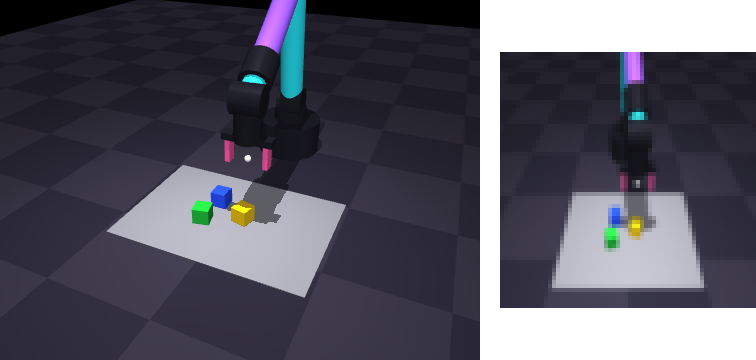
\includegraphics[width=0.9\linewidth]{scene.png}
\caption{Слева~--- сцена: рука (из проекта ARMageddon) и три цветных блока. Справа~--- всё,
что видит робот: картинка $64{\times}64$. Плюс инструкция вида <<grab the blue block>>.}
\end{figure}

\begin{itemize}
\item \textbf{40 сцен}, в каждой 3 блока из 4 цветов на своих местах (с небольшим случайным сдвигом).
\item \textbf{Обычная сцена} показана всегда с одной целью (30 демонстраций). \textbf{Контрастная}~---
со всеми тремя целями (по 10). Цели обычных сцен сбалансированы по цветам, чтобы правило
<<всегда бери красный>> не работало.
\item \textbf{6 условий}: $f = 0,\ 0.05,\ 0.1,\ 0.25,\ 0.5,\ 1$. В каждом \textbf{ровно 1200 демонстраций}.
\item \textbf{Модель}: свёрточная сеть + язык через FiLM от замороженного энкодера MiniLM,
предсказание пачки из 5 действий (как в ACT~\citep{zhao2023act}). Рецепт обучения одинаковый везде.
\item \textbf{Проверка}: в сценах 20--39 (обычных во всех условиях до $f=0.5$) просим блок,
который в этой сцене \emph{ни разу} не просили. Смотрим, на каком блоке робот сомкнёт пальцы.
\item \textbf{3 сида} на условие, 660 эпизодов проверки на каждую обученную политику,
бутстреп-интервалы и логистическая регрессия.
\end{itemize}

\begin{figure}[h]
\centering
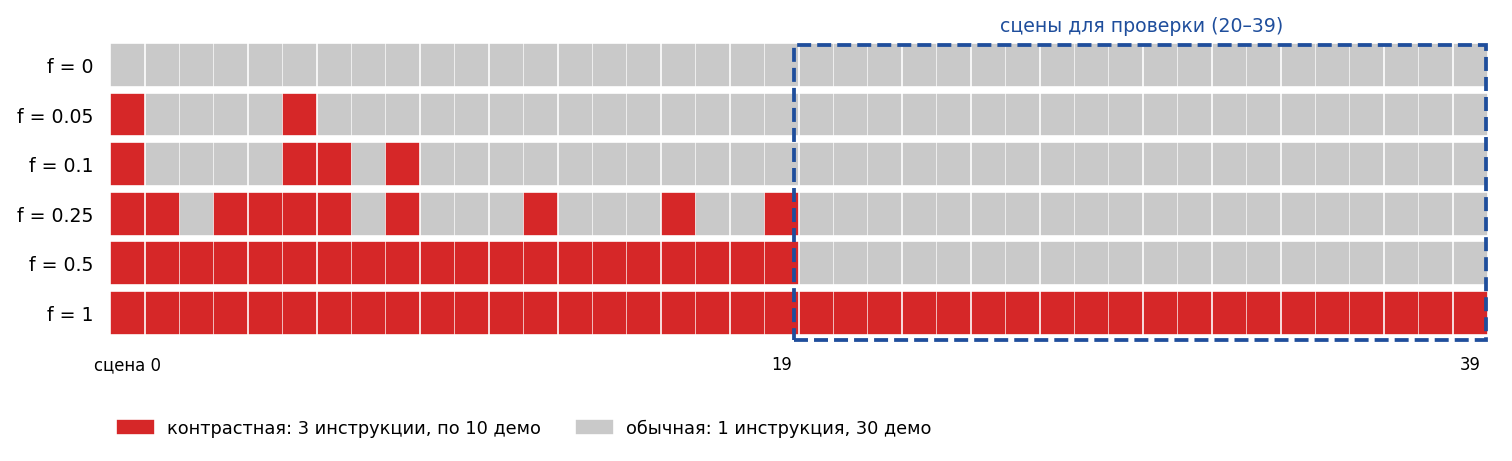
\includegraphics[width=\linewidth]{design.png}
\caption{Какие сцены контрастные в каждом условии. Наборы вложены друг в друга, а сцены 20--39
используются для проверки.}
\end{figure}

\section{Что уже есть}

\begin{tabular}{ll}
Поиск литературы и проверка новизны & \done \\
Пререгистрация (git, до экспериментов) & \done \\
Сцена, скриптовый эксперт (30/30 успешно), пул из 3600 демонстраций & \done \\
Модель, обучение, оценка, 15 тестов дизайна & \done \\
Пилот (2 политики) & \done \\
Основной эксперимент: 18 обучений & \running \\
Эксперимент E (4 сцены вместо 40) & \todo \\
Статистика, графики, статья в \LaTeX, репозиторий на GitHub & \todo \\
\end{tabular}

\subsection*{Пилот: первая проблема и первая неожиданность}

Сначала робот доезжал до блока с точностью 2\,мм, но \emph{никогда не сжимал пальцы}. Моменты
<<доехал>> и <<начинаю сжимать>> для камеры выглядят одинаково, и сеть застревала посередине.
Лечится temporal ensembling (усреднением будущих предсказаний, как в ACT). Это изменение
разрешено пререгистрацией на этапе пилота и задокументировано.

\begin{table}[h]
\centering\small
\begin{tabular}{lcccc}
\toprule
Пилот (отдельный сид) & \makecell{берёт\\названный блок} & \makecell{берёт\\<<привычный>>} & \makecell{не берёт\\ничего} & \makecell{обычная\\задача} \\
\midrule
$f=0$ (контраста нет) & 57\% & 3\% & 40\% & 86\% \\
$f=1$ (всё контрастное) & 88\% & 0\% & 12\% & 82\% \\
\bottomrule
\end{tabular}
\caption{Пилот. Неожиданность: без контраста робот почти \emph{не} берёт <<привычный>> блок, а
либо слушается, либо теряется. В статистику гипотез пилот не входит.}
\end{table}

Наше объяснение: в этом дизайне связать слово <<red>> с красным цветом \emph{проще}, чем
запомнить нужный блок в каждой из 40 сцен, поэтому коротким путём становится сам язык.
Если это так, то <<глухота>> к языку зависит от того, \emph{что сети легче выучить}~--- сцену или
слово. Для проверки добавлен \textbf{эксперимент E}: всего 4 сцены (как в LIBERO, где сцен мало),
где запомнить сцену легко. Он записан в пререгистрацию \emph{до} результатов основного
эксперимента и помечен как разведочный.

\subsection*{Попутная находка: энкодер сам <<глуховат>>}

Готовый языковой энкодер MiniLM считает <<pick up the red block>> ближе к <<pick up the blue
block>>, чем к <<grab the red cube>>. В его векторе \textbf{цвет объясняет лишь 32\% разброса,
а формулировка фразы~--- 66\%}. То есть заметная часть <<глухоты>> может начинаться ещё до
робота, в самом представлении текста.

\section{Почему это важно}

\begin{itemize}
\item \textbf{Наука}: первая \emph{причинная} проверка того, почему VLA не слушают язык.
\item \textbf{Практика}: сбор данных для роботов~--- самая дорогая часть. Ответ <<добавь X\%
контрастных демонстраций>>~--- прямой рецепт для лабораторий и компаний.
\item \textbf{Любой исход полезен}: если слушание обобщается, это рецепт; если нет, это важное
ограничение, которое надо знать.
\end{itemize}

\section{Что дальше}

\begin{enumerate}
\item Досчитать основной эксперимент (около 2 часов) и эксперимент E (около часа).
\item Статистика по пререгистрированному плану, графики <<доза--эффект>>.
\item Статья в формате arXiv (на английском) и открытый репозиторий: код, пререгистрация
с историей коммитов, записи каждого эпизода.
\end{enumerate}

\bibliographystyle{plainnat}
\bibliography{../paper/refs}
\end{document}
